
1 \documentclass[preview]{standalone}
\usepackage[a4paper, portrait, hmargin=5.5cm,vmargin=0cm]{geometry}
\usepackage{tikz}

\def\width{10}
\def\height{10}

\def\minorcolor{black!30!white}
\def\majorcolor{black!90!white}

% \tikzstyle{backtrack}=[rectangle,draw=black,fill=white,inner sep=12pt,minimum height=32pt, minimum width=20mm]

% \tikzstyle{minorgrid/.style={minorcolor, very thin}}
% \tikzstyle{majorgrid/.style={majorcolor, thin}}


\begin{document}

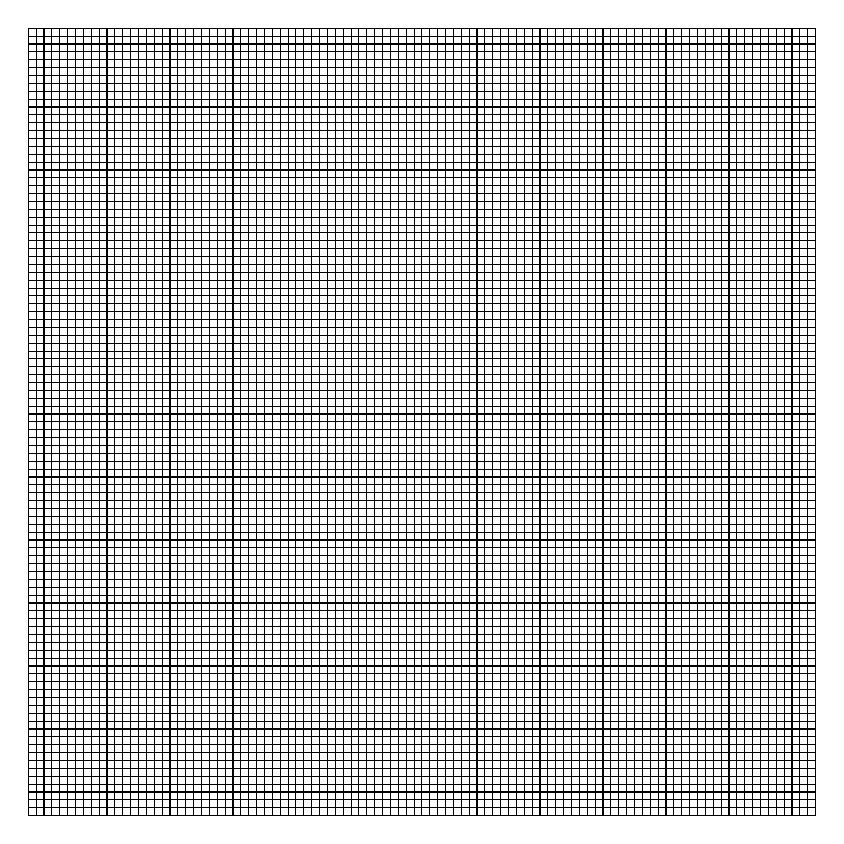
\begin{tikzpicture}[x=1cm, y=1cm]
  \draw[step=1mm] (0,0) grid (\width,\height);
%   \draw[step=5mm, line width=0.2mm, black!40!white] (0,0) grid (\width,\height);
%   \draw[step=5cm, line width=0.3mm, black!50!white] (0,0) grid (\width,\height);
%   \draw[step=1cm, line width=0.3mm, black!90!white] (0,0) grid (\width,\height);
\end{tikzpicture}

\end{document}


